% One figure, four slides: each overlay command shows up on its own.
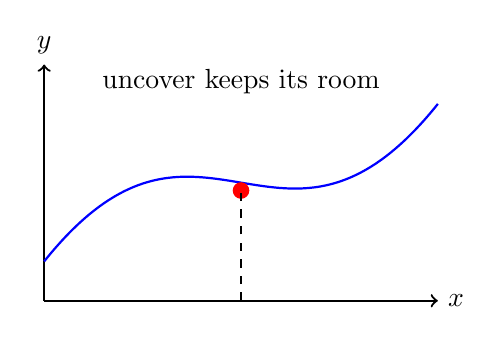
\begin{tikzpicture}
  \draw[->, thick] (0,0) -- (5,0) node[right] {$x$};
  \draw[->, thick] (0,0) -- (0,3) node[above] {$y$};
  \pause
  \draw[blue, thick] (0,0.5) .. controls (2,3) and (3,0) .. (5,2.5);
  \uncover<3->{\node[above] at (2.5,2.5) {uncover keeps its room};}
  \only<4>{\fill[red] (2.5,1.4) circle (3pt);}
  \draw<4>[dashed] (2.5,0) -- (2.5,1.4);
\end{tikzpicture}
